    \expectedproblemsection{Reasoning and Puzzle Problems}

    \begin{expectedproblem}[Sum-and-Product Puzzle]
        Two integers $x$ and $y$ satisfy
        \[
            1<x<y,
            \qquad
            x+y\leq100.
        \]
        The sum $x+y$ is disclosed privately to $S$, and the product $xy$ is
        disclosed privately to $P$. The preceding information is common
        knowledge. The following conversation then takes place:
        \begin{problemchoices}
            \item $P$: ``I do not know the pair.''
            \item $S$: ``I knew that you did not know the pair.''
            \item $P$: ``Now I know the pair.''
            \item $S$: ``Now I also know the pair.''
        \end{problemchoices}
        Determine $(x,y)$.
    \end{expectedproblem}

    \begin{solution}
        Let
        \[
            \Omega_0
            =
            \{(x,y)\in\N^2\mid (1<x<y)\land(x+y\leq100)\}.
        \]
        For $\Omega\subseteq\Omega_0$ and $\omega=(x,y)\in\Omega$, define the
        information sets
        \[
            \mathcal{I}_S^\Omega(\omega)
            =
            \{(u,v)\in\Omega\mid u+v=x+y\},
        \]
        \[
            \mathcal{I}_P^\Omega(\omega)
            =
            \{(u,v)\in\Omega\mid uv=xy\}.
        \]
        The four announcements successively restrict the state space as follows:
        \[
            \Omega_1
            =
            \{\omega\in\Omega_0\mid
              |\mathcal{I}_P^{\Omega_0}(\omega)|>1\},
        \]
        \[
            \Omega_2
            =
            \{\omega\in\Omega_1\mid
              \mathcal{I}_S^{\Omega_0}(\omega)\subseteq\Omega_1\},
        \]
        \[
            \Omega_3
            =
            \{\omega\in\Omega_2\mid
              |\mathcal{I}_P^{\Omega_2}(\omega)|=1\},
        \]
        and
        \[
            \Omega_4
            =
            \{\omega\in\Omega_3\mid
              |\mathcal{I}_S^{\Omega_3}(\omega)|=1\}.
        \]

        The finite elimination is summarized by
        \[
            \begin{array}{c|l|c}
                \text{stage} & \text{public information retained} &
                \text{number of states}\\
                \hline
                0 & (1<x<y)\land(x+y\leq100) & 2352\\
                1 & P\text{ does not know the pair} & 1747\\
                2 & S\text{ knew that }P\text{ did not know} & 145\\
                3 & P\text{ now knows the pair} & 86\\
                4 & S\text{ now knows the pair} & 1
            \end{array}
        \]
        At the second stage, the possible sums are exactly
        \[
            11,\ 17,\ 23,\ 27,\ 29,\ 35,\ 37,\ 41,\ 47,\ 53.
        \]
        These values follow by checking, for each admissible sum, whether every
        compatible factorization has at least two representations in
        $\Omega_0$. After the third announcement, the only sum-information set
        of cardinality $1$ is
        \[
            \mathcal{I}_S^{\Omega_3}(4,13)=\{(4,13)\}.
        \]
        Therefore,
        \[
            \Omega_4=\{(4,13)\},
        \]
        and the unique pair is
        \[
            \boxed{(x,y)=(4,13)}.
        \]
    \end{solution}

    \begin{expectedproblem}[Bertrand's Box Paradox]
        Three boxes contain coins as follows:
        \[
            GG,\qquad GS,\qquad SS,
        \]
        where $G$ denotes a gold coin and $S$ denotes a silver coin. A box is
        chosen uniformly at random, and then one of its two coins is chosen
        uniformly at random. The chosen coin is gold. Determine the
        conditional probability that the other coin in the same box is also
        gold.
    \end{expectedproblem}

    \begin{solution}
        Let $B_{GG}$ be the event that the chosen box is $GG$, and let $G$ be
        the event that the observed coin is gold. Then
        \[
            \Prob(G\mid B_{GG})=1,
            \qquad
            \Prob(G\mid B_{GS})=\frac12,
            \qquad
            \Prob(G\mid B_{SS})=0.
        \]
        Since the three boxes are initially equally likely, Bayes' theorem
        gives
        \[
            \begin{aligned}
                \Prob(B_{GG}\mid G)
                &=
                \frac{
                    \Prob(G\mid B_{GG})\Prob(B_{GG})
                }{
                    \Prob(G\mid B_{GG})\Prob(B_{GG})
                    +
                    \Prob(G\mid B_{GS})\Prob(B_{GS})
                }\\
                &=
                \frac{1\cdot(1/3)}
                {1\cdot(1/3)+(1/2)\cdot(1/3)}
                =
                \boxed{\frac23}.
            \end{aligned}
        \]
        Equivalently, after observing gold, the selected coin is equally
        likely to be any of the three gold coins present among the boxes.
        Two of those three coins lie in the $GG$ box.
    \end{solution}

    \begin{expectedproblem}[Penney's Game]
        The first player chooses a pattern of three coin tosses, such as
        $\mathrm{HHT}$. After seeing this choice, the second player chooses a
        different pattern of length $3$. A fair coin is then tossed repeatedly
        until one of the two patterns first appears as three consecutive
        outcomes; the player who chose that pattern wins.

        Prove that the second player can always choose a pattern whose winning
        probability is greater than $1/2$.
    \end{expectedproblem}

    \begin{solution}
        For two patterns $X$ and $Y$ of length $3$, define the overlap score
        \[
            C(X,Y)
            =
            \sum_{\substack{1\leq k\leq3\\
            \text{suffix}_k(X)=\text{prefix}_k(Y)}}2^k.
        \]
        A standard fair-betting argument gives the probability that $Y$ occurs
        before $X$:
        \[
            \Prob(Y\text{ before }X)
            =
            \frac{C(X,X)-C(X,Y)}
            {C(X,X)-C(X,Y)+C(Y,Y)-C(Y,X)}.
        \]
        Indeed, start a new unit-stake gambler before each toss, with one team
        betting successively on $X$ and the other on $Y$, doubling its capital
        after each correct fair bet. At the stopping time, the surviving
        capital of the team betting on $Y$ is $C(X,Y)$ if $X$ wins and
        $C(Y,Y)$ if $Y$ wins; the analogous statement holds for the other
        team. Equality of the two expected net gains yields the displayed
        formula.

        Write the first player's pattern as
        \[
            X=x_1x_2x_3,
        \]
        and let $\overline{x_2}$ denote the opposite face of $x_2$. The second
        player chooses
        \[
            Y=\overline{x_2}x_1x_2.
        \]
        By interchanging heads and tails if necessary, it is enough to check
        the following four cases:
        \[
            \begin{array}{c|c|c}
                X & Y & \Prob(Y\text{ before }X)\\
                \hline
                \mathrm{HHH} & \mathrm{THH} & 7/8\\
                \mathrm{HHT} & \mathrm{THH} & 3/4\\
                \mathrm{HTH} & \mathrm{HHT} & 2/3\\
                \mathrm{HTT} & \mathrm{HHT} & 2/3
            \end{array}
        \]
        These values follow immediately from the overlap formula. Each is
        strictly greater than $1/2$, so the second player always has the
        required choice.
    \end{solution}

    \begin{expectedproblem}[Josephus Problem]
        The people numbered
        \[
            1,2,\ldots,n
        \]
        stand in a circle. Starting with person $1$, count repeatedly around
        the circle and eliminate every second person. After each elimination,
        resume counting with the next remaining person. Determine the number
        of the last survivor.
    \end{expectedproblem}

    \begin{solution}
        Let $J(n)$ denote the number of the survivor. If $n=2m$, the first
        circuit eliminates all even-numbered people. Relabeling the survivors
        \[
            1,3,\ldots,2m-1
        \]
        as $1,2,\ldots,m$ gives
        \[
            J(2m)=2J(m)-1.
        \]
        A similar relabeling when $n=2m+1$ gives
        \[
            J(2m+1)=2J(m)+1.
        \]

        Write
        \[
            n=2^r+\ell,
            \qquad
            0\leq\ell<2^r.
        \]
        Starting from $J(2^r)=1$, a strong induction using these recurrences
        yields
        \[
            \boxed{J(n)=2\ell+1}.
        \]
        In binary notation this has a particularly simple interpretation. If
        \[
            n=(1b_{r-1}b_{r-2}\cdots b_0)_2,
        \]
        then
        \[
            J(n)=(b_{r-1}b_{r-2}\cdots b_0 1)_2;
        \]
        the leading binary digit of $n$ is moved to the end.
    \end{solution}

    \begin{expectedproblem}[Conway's Soldiers]
        On an infinite square grid, every square on or below a fixed horizontal
        line initially contains a soldier, and every square strictly above the
        line is empty. A legal move jumps one soldier horizontally or
        vertically over an adjacent soldier into the next square, which must be
        empty; the jumped soldier is removed. Prove that no soldier can reach
        the fifth row above the initial line.
    \end{expectedproblem}

    \begin{solution}
        Fix a target square $T$ in the fifth row and put
        \[
            q=\frac{\sqrt5-1}{2},
            \qquad
            q+q^2=1.
        \]
        Give each square $Q$ the weight
        \[
            w(Q)=q^{d(Q,T)},
        \]
        where $d$ is the Manhattan distance, and let $W$ be the sum of the
        weights of all occupied squares.

        Consider three consecutive squares in the direction of a legal jump.
        Their distances from $T$ have one of the forms
        \[
            (m+2,m+1,m),
            \qquad
            (m,m+1,m+2),
            \qquad
            (m+1,m,m+1).
        \]
        In the first case, the jump moves toward $T$ and
        \[
            q^{m+2}+q^{m+1}=q^m
        \]
        because $q+q^2=1$. In the second case,
        $q^m+q^{m+1}>q^{m+2}$, and in the third case,
        $q^{m+1}+q^m>q^{m+1}$. Thus no legal move increases $W$.

        Take the initial boundary to be $y=0$ and $T=(0,5)$. The initial weight
        is
        \[
            \begin{aligned}
                W_0
                &=
                \sum_{m=0}^{\infty}\sum_{k\in\Z}q^{|k|+m+5}\\
                &=
                q^5
                \left(1+2\sum_{k=1}^{\infty}q^k\right)
                \left(\sum_{m=0}^{\infty}q^m\right)
                =1.
            \end{aligned}
        \]

        Before a soldier could first reach $T$, only finitely many moves would
        have occurred. Hence only finitely many initially occupied squares
        could have been altered, so at least one untouched soldier of positive
        weight would remain. If $T$ were occupied, it alone would contribute
        weight $1$, and the untouched soldier would contribute an additional
        positive amount. This would give $W>1$, contradicting $W\leq W_0=1$.

        Therefore no soldier can reach the fifth row.
    \end{solution}

    \begin{expectedproblem}[Three Utilities Problem]
        Three houses and three utility companies---water, gas, and
        electricity---are represented by six distinct points in the plane. Is
        it possible to join every house to every utility company by curves so
        that no two curves intersect and no curve passes through any of the six
        points other than its endpoints? Prove the answer.
    \end{expectedproblem}

    \begin{solution}
        Such a drawing would be a planar embedding of the complete bipartite
        graph $K_{3,3}$. This graph has
        \[
            V=6,
            \qquad
            E=9.
        \]

        The graph $K_{3,3}$ is simple, bipartite, and has no bridges. Thus every
        face boundary in a planar embedding would be a closed walk of length at
        least $4$. If $F$ is the number of faces, double counting edge--face
        incidences gives
        \[
            2E\geq4F,
            \qquad\text{so}\qquad
            F\leq\frac{E}{2}.
        \]
        Euler's formula would then give
        \[
            2=V-E+F
            \leq
            V-E+\frac{E}{2},
        \]
        and hence
        \[
            E\leq2V-4.
        \]
        For $K_{3,3}$ this would require
        \[
            9\leq2\cdot6-4=8,
        \]
        which is impossible. Thus the requested system of nonintersecting
        connections cannot be drawn in the plane.
    \end{solution}

    \begin{expectedproblem}[Seven Bridges of K\"onigsberg]
        The city of K\"onigsberg was divided by the Pregel River into four land
        masses, connected by seven bridges as shown below. Is it possible to
        start at one land mass, cross each bridge exactly once, and end at some
        land mass? Prove your answer.

        \begin{center}
            
\includegraphics[
                width=0.42\textwidth
            ]{Figures/ReasoningandPuzzleProblems/SevenBridgesofKonigsberg/ProblemFigure.pdf}
        \end{center}
    \end{expectedproblem}

    \begin{solution}
        Replace each land mass by a vertex and each bridge by an edge. Then the
        problem becomes the following graph-theoretic question: does the
        resulting connected multigraph have an Euler trail, that is, a trail
        using every edge exactly once?

        In the graph above, the four vertex degrees are
        \[
            3,\quad 3,\quad 3,\quad 5.
        \]
        In particular, all four vertices have odd degree.

        A connected graph has an Euler trail if and only if it has exactly zero
        or two vertices of odd degree. Since this graph has four odd vertices,
        an Euler trail does not exist.

        Therefore it is impossible to cross each of the seven bridges exactly
        once.
    \end{solution}

    \begin{expectedproblem}[15 Puzzle]
        In the standard fifteen puzzle, a legal move consists of sliding one
        tile adjacent to the blank square into the blank square. Starting from
        the solved position on the left, determine whether one can reach the
        position on the right, in which only the tiles $14$ and $15$ have been
        interchanged.

        \begin{center}
            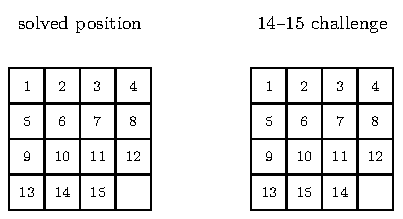
\includegraphics[
                width=0.72\textwidth
            ]{Figures/ReasoningandPuzzleProblems/FifteenPuzzle1415Challenge/ProblemFigure.pdf}
        \end{center}
    \end{expectedproblem}

    \begin{solution}
        Read the tiles row by row from left to right and top to bottom, omitting
        the blank square. Let $I$ be the number of inversions in this resulting
        list, and let $r$ be the row number of the blank square counted from the
        top. We claim that the parity of
        \[
            I+r
        \]
        is invariant under every legal move.

        If the blank square moves horizontally, then the order of the numbered
        tiles in the row-by-row list does not change, so $I$ is unchanged, and
        $r$ is also unchanged. Hence the parity of $I+r$ is unchanged.

        If the blank square moves vertically, then one tile moves up or down by
        one row. In the row-by-row list, that tile passes across exactly three
        other tiles, so the inversion number changes by $3$, and therefore its
        parity changes. At the same time, the blank square moves to an adjacent
        row, so the parity of $r$ also changes. Hence the parity of $I+r$
        remains unchanged in this case as well.

        In the solved position, the inversion number is
        \[
            I=0,
        \]
        and the blank square lies in row $4$, so
        \[
            I+r\equiv0+4\equiv0\pmod2.
        \]
        In the target position, the list differs only by the transposition of
        $14$ and $15$, so
        \[
            I=1,
        \]
        while the blank square is still in row $4$. Thus
        \[
            I+r\equiv1+4\equiv1\pmod2.
        \]
        Since the parity of $I+r$ is invariant, the target position cannot be
        reached from the solved position.

        Therefore the 14--15 challenge is impossible.
    \end{solution}

    \begin{expectedproblem}[Chomp]
        An $m\times n$ rectangular chocolate bar consists of unit-square
        pieces. The lower-left piece is poisoned.

        On each turn, a player chooses one remaining piece and eats that piece
        together with every remaining piece weakly above it and weakly to its
        right. The player who eats the poisoned piece loses.

        Prove that whenever the initial bar contains more than the poisoned
        piece alone, the first player has a winning strategy.
    \end{expectedproblem}

    \begin{solution}
        Since the game is finite and has no draws, one of the two players has a
        winning strategy. Suppose, for contradiction, that the second player
        has one.

        Let the first player eat only the upper-right corner piece. According
        to the supposed winning strategy, the second player must have a
        non-poisoned response; otherwise the second player is forced to eat the
        poisoned piece and loses. Let that response be a remaining piece $C$.
        Eating $C$ also removes the upper-right corner, because that corner
        lies above and to the right of $C$. Hence the position obtained after
        these two moves is exactly the position that would have resulted had
        the first player chosen $C$ on the very first move.

        After the original two-move sequence, this position is losing for the
        player whose turn it is, namely the first player. The first player
        could instead begin by choosing $C$ and hand the identical losing
        position to the second player. This contradicts the assumption that
        the second player has a winning strategy.

        Therefore the first player has a winning strategy. The argument proves
        its existence without identifying the winning first move in general.
    \end{solution}

    \begin{expectedproblem}[Braess's Paradox]
        A total traffic flow of $4000$ units travels from $S$ to $T$ in the
        directed network with routes
        \[
            S\to A\to T
            \qquad\text{and}\qquad
            S\to B\to T.
        \]
        If $x$ denotes the flow on a road, its travel time is given by
        \[
            \begin{array}{c|cccc}
                \text{Road}
                & S\to A & A\to T & S\to B & B\to T\\
                \hline
                \text{Travel time}
                & x/100 & 45 & 45 & x/100
            \end{array}
        \]
        Each driver chooses a route of minimum travel time, taking the total
        road flows as given.

        Determine the equilibrium travel time in the original network. Then a
        new directed road $A\to B$ with travel time $0$ is added. Determine the
        new equilibrium travel time.
    \end{expectedproblem}

    \begin{solution}
        Let $y$ units use the upper route $S\to A\to T$. Then $4000-y$
        units use the lower route, and their travel times are
        \[
            C_U(y)=\frac{y}{100}+45,
            \qquad
            C_L(y)=45+\frac{4000-y}{100}.
        \]
        At equilibrium both routes are used and have equal travel time. Thus
        \[
            \frac{y}{100}+45
            =
            45+\frac{4000-y}{100},
        \]
        so $y=2000$ and
        \[
            C_U=C_L=65.
        \]

        After the road $A\to B$ is added, let $f$, $g$, and $h$ be the flows on
        the routes
        \[
            S\to A\to T,
            \qquad
            S\to B\to T,
            \qquad
            S\to A\to B\to T,
        \]
        respectively. Put
        \[
            x=f+h,
            \qquad
            z=g+h,
        \]
        for the flows on $S\to A$ and $B\to T$. The three route costs are
        \[
            C_U=\frac{x}{100}+45,
            \qquad
            C_L=45+\frac{z}{100},
            \qquad
            C_M=\frac{x+z}{100}.
        \]
        If $f>0$, equilibrium would require $C_U\leq C_M$, which implies
        $z\geq4500$, impossible because the total flow is $4000$. Hence
        $f=0$. Similarly, $g=0$. Therefore
        \[
            h=4000,
            \qquad
            x=z=4000,
        \]
        and every driver uses the new middle route with travel time
        \[
            C_M=40+40=80.
        \]
        Thus adding the zero-time road increases the equilibrium travel time
        from
        \[
            \boxed{65}
            \qquad\text{to}\qquad
            \boxed{80}.
        \]
    \end{solution}

    \begin{expectedproblem}[100 Prisoners and 100 Boxes]
        One hundred prisoners and one hundred boxes are labeled
        $1,2,\ldots,100$. The prisoners' labels are placed in the boxes
        according to a uniformly random permutation.

        The prisoners enter the room one at a time. Each prisoner may open at
        most $50$ boxes and must restore them before leaving. They may agree on
        a strategy beforehand but may not communicate after the process
        begins. They all survive if and only if every prisoner finds their own
        label.

        Find a strategy whose probability of saving all the prisoners is
        greater than $30\%$.
    \end{expectedproblem}

    \begin{solution}
        Regard the contents of the boxes as a permutation $\pi$ of
        $\{1,2,\ldots,100\}$, where box $i$ contains the label $\pi(i)$.
        Prisoner $i$ first opens box $i$. If it contains label $j$, the
        prisoner next opens box $j$, and continues following the labels in
        this way for at most $50$ boxes.

        This procedure follows the cycle of $\pi$ containing $i$. Therefore
        every prisoner finds their own label if and only if every cycle of
        $\pi$ has length at most $50$.

        For $51\leq k\leq100$, the probability that a uniformly random
        permutation contains a $k$-cycle is $1/k$. Moreover, two cycles of
        lengths greater than $50$ cannot occur simultaneously. Hence the
        probability that some cycle is too long is
        \[
            \sum_{k=51}^{100}\frac{1}{k}.
        \]
        The probability that all prisoners survive is therefore
        \[
            1-\sum_{k=51}^{100}\frac{1}{k}
            =
            1-\bigl(H_{100}-H_{50}\bigr)
            \approx
            0.3118278207.
        \]
        Thus the cycle-following strategy saves all the prisoners with
        probability approximately
        \[
            \boxed{31.18\%},
        \]
        which is greater than $30\%$.
    \end{solution}

    \begin{expectedproblem}[St.\ Petersburg Paradox]
        A fair coin is tossed until heads appears for the first time. If the
        first head appears on the $n$th toss, the player receives
        \[
            2^n
        \]
        units of money. Compute the expected payoff. If decisions are based
        only on expected monetary value, determine how large an entry fee it
        would be rational to pay, and explain why the conclusion is regarded
        as paradoxical.
    \end{expectedproblem}

    \begin{solution}
        The probability that the first head appears on the $n$th toss is
        \[
            \left(\frac12\right)^n.
        \]
        Therefore the expected payoff is
        \[
            \Exp[X]
            =
            \sum_{n=1}^{\infty}
            2^n\left(\frac12\right)^n
            =
            \sum_{n=1}^{\infty}1
            =
            \boxed{\infty}.
        \]
        Under the rule of maximizing expected monetary value alone, subtracting
        any finite entry fee still leaves an infinite expected net payoff.
        Thus there is no finite upper bound on the fee that this rule recommends.

        The conclusion conflicts sharply with ordinary judgment. For example,
        the payoff is at most $2$ with probability $1/2$ and at most $4$ with
        probability $3/4$, so most outcomes are small. The infinite expectation
        is driven by extremely rare but extremely large prizes. This mismatch
        shows that expected monetary value alone is not always an adequate
        decision criterion; finite resources, risk, and diminishing marginal
        utility of money can all change a rational valuation.
    \end{solution}

    \begin{expectedproblem}[Bachet's Weights Problem]
        Using a two-pan balance and weights of positive integer numbers of
        pounds, determine the minimum number of weights needed to weigh every
        integer load from $1$ to $40$ pounds. A weight may be placed on either
        pan. Determine the weights as well.
    \end{expectedproblem}

    \begin{solution}
        With $m$ weights, each weight has three possible roles: on the load pan,
        unused, or on the opposite pan. Hence at most $3^m$ signed sums can be
        produced. These include $0$ and occur in opposite pairs, so at most
        \[
            \frac{3^m-1}{2}
        \]
        positive loads can be distinguished. To cover $1,2,\ldots,40$, we need
        \[
            \frac{3^m-1}{2}\geq40,
        \]
        and therefore $m\geq4$.

        Four weights suffice: take
        \[
            \boxed{1,3,9,27}.
        \]
        Every integer from $-40$ to $40$ has a balanced ternary representation
        \[
            N=\varepsilon_0+3\varepsilon_1+9\varepsilon_2+27\varepsilon_3,
            \qquad
            \varepsilon_i\in\{-1,0,1\}.
        \]
        A coefficient $1$ places the corresponding weight opposite the load,
        a coefficient $-1$ places it with the load, and a coefficient $0$
        leaves it unused. Thus all loads from $1$ through $40$ can be weighed,
        and four weights are minimal.
    \end{solution}

    \begin{expectedproblem}[Hex]
        On a finite $n\times n$ Hex board, two players alternately place stones
        of their own colors in empty cells. Each player wins by forming a
        connected path joining a designated pair of opposite sides. Prove that
        the first player has a winning strategy.
    \end{expectedproblem}

    \begin{solution}
        A completely filled Hex board cannot be a draw. Indeed, consider the
        component of one color attached to one of its target sides. If that
        component does not reach the opposite target side, its boundary across
        the hexagonal cells produces a connected chain of the other color
        between the other pair of opposite sides. Thus exactly one player has a
        winning connection when the board is full.

        Since the game is finite and has no draws, one of the two players has a
        winning strategy. Suppose, for contradiction, that the second player
        has one. The first player places a stone in any cell and thereafter
        follows the supposed second-player strategy, using the symmetry that
        interchanges the two colors and their target sides. If the strategy ever
        calls for the already occupied initial cell, the first player makes any
        legal move instead and continues.

        An extra stone of one's own color can never destroy a connection, so
        this stolen strategy still wins. That contradicts the assumption that
        the second player had a winning strategy. Hence the first player has
        one. The argument is nonconstructive and need not identify a winning
        opening move.
    \end{solution}

    \begin{expectedproblem}[Secretary Problem]
        There are $n\geq2$ applicants with distinct ranks, presented in a
        uniformly random order. After each interview, the current applicant must be
        accepted or rejected permanently. Only the relative ranking of the
        applicants seen so far is known. Determine a strategy maximizing the
        probability of selecting the best applicant, and find its asymptotic
        success probability as $n\to\infty$.
    \end{expectedproblem}

    \begin{solution}
        Only an applicant who is best among those seen so far can be accepted
        optimally. The optimal rule has a threshold form: reject the first $r$
        applicants, then accept the first subsequent applicant who is better
        than all of the first $r$.

        For a fixed $r$, the best applicant must occur at some position
        $k>r$, and then the best among the first $k-1$ applicants must lie among
        the first $r$. Therefore the success probability is
        \[
            P_n(r)
            =
            \sum_{k=r+1}^{n}
            \frac{1}{n}\frac{r}{k-1}
            =
            \frac{r}{n}
            \sum_{j=r}^{n-1}\frac{1}{j}.
        \]
        Moreover,
        \[
            n\bigl(P_n(r+1)-P_n(r)\bigr)
            =
            \sum_{j=r+1}^{n-1}\frac{1}{j}-1.
        \]
        Hence $P_n(r)$ increases until the displayed harmonic tail passes
        below $1$ and then decreases. Thus an optimal cutoff is the integer
        where that crossing occurs.

        Since
        \[
            \sum_{j=r}^{n-1}\frac{1}{j}
            =
            \ln\left(\frac{n}{r}\right)+o(1),
        \]
        the optimal cutoff satisfies
        \[
            \frac{r}{n}\to\frac{1}{e}.
        \]
        Substitution in $P_n(r)$ gives the limiting success probability
        \[
            \boxed{\frac{1}{e}}.
        \]
    \end{solution}

    \begin{expectedproblem}[Nim, Bouton's Theorem]
        Several heaps contain
        \[
            a_1,a_2,\ldots,a_m
        \]
        stones. Two players alternately choose one heap and remove any positive
        number of stones from it. The player taking the last stone wins.
        Characterize the positions from which the next player has a winning
        strategy.
    \end{expectedproblem}

    \begin{solution}
        Let
        \[
            s=a_1\oplus a_2\oplus\cdots\oplus a_m
        \]
        be the bitwise XOR, or nim-sum, of the heap sizes.

        Suppose first that $s=0$. Any legal move changes one heap from $a_i$ to
        a smaller value $b_i$. At the highest binary digit where $a_i$ and
        $b_i$ differ, the new nim-sum has a $1$, so every move leads to a
        position with nonzero nim-sum.

        Now suppose that $s\neq0$. Choose the highest binary digit in which $s$
        has a $1$. Some heap $a_i$ also has a $1$ in that position. Set
        \[
            b_i=a_i\oplus s.
        \]
        At the highest chosen digit, $b_i$ has $0$ while $a_i$ has $1$, so
        $b_i<a_i$ and this is a legal reduction. The new nim-sum is
        \[
            s\oplus a_i\oplus b_i=0.
        \]

        Thus every nonzero nim-sum position can move to a zero nim-sum
        position, while every move from a zero nim-sum position makes it
        nonzero. Therefore
        \[
            \boxed{
                a_1\oplus\cdots\oplus a_m\neq0
                \text{ exactly for the next-player winning positions}
            }.
        \]
    \end{solution}

    \begin{expectedproblem}[100 Prisoners and a Light Bulb]
        One hundred prisoners are isolated. Each day, one prisoner is selected
        independently and uniformly at random and taken to a room containing a
        light bulb, initially off. A prisoner in the room may inspect and change
        the bulb. Before the process begins, the prisoners may agree on a
        strategy. At any visit, a prisoner may declare that everyone has visited
        the room; a correct declaration frees all prisoners, while an incorrect
        one kills them. Find a strategy that eventually permits a correct
        declaration with probability $1$.
    \end{expectedproblem}

    \begin{solution}
        Designate one prisoner as the counter. Each of the other $99$ prisoners
        follows this rule: the first time that prisoner enters and finds the
        bulb off, turn it on; after having done so once, never turn it on again.

        The counter never turns the bulb on. Whenever the counter enters and
        finds it on, the counter turns it off and increases a private count by
        $1$. When the count reaches $99$, the counter declares that everyone
        has visited.

        Every counted signal was produced by a different non-counter, so the
        declaration is certainly correct. Under independent uniform random
        selection, every prisoner is selected infinitely often with probability
        $1$. Consequently, each uncounted prisoner eventually encounters an off
        bulb and signals, and the counter eventually records every signal.
        Thus the correct declaration occurs with probability $1$.
    \end{solution}

    \begin{expectedproblem}[Sicherman Dice]
        Label the six faces of each of two dice by positive integers, allowing
        repeated labels. Find a pair of dice, not both standard, whose sum has
        exactly the same probability distribution as the sum of two standard
        dice.
    \end{expectedproblem}

    \begin{solution}
        For a die with face labels $d_1,\ldots,d_6$, encode its sums by the
        polynomial
        \[
            P(x)=x^{d_1}+\cdots+x^{d_6}.
        \]
        The coefficient of $x^k$ in the product of the two dice polynomials is
        the number of outcomes with sum $k$.

        Take dice with labels
        \[
            \boxed{1,2,2,3,3,4}
        \]
        and
        \[
            \boxed{1,3,4,5,6,8}.
        \]
        Their polynomials are
        \[
            P(x)=x+2x^2+2x^3+x^4
        \]
        and
        \[
            Q(x)=x+x^3+x^4+x^5+x^6+x^8.
        \]
        Direct factorization gives
        \[
            P(x)Q(x)
            =
            (x+x^2+x^3+x^4+x^5+x^6)^2.
        \]
        Hence every possible sum occurs with exactly the same multiplicity as
        for two standard dice.
    \end{solution}

    \begin{expectedproblem}[Number Erasing Game]
        The integers
        \[
            1,2,\ldots,100
        \]
        are written on a board. Repeatedly erase two numbers $a,b$ and replace
        them by
        \[
            a+b+ab.
        \]
        Determine the final number and prove that it is independent of all
        choices.
    \end{expectedproblem}

    \begin{solution}
        The operation is designed so that
        \[
            (a+b+ab)+1=(a+1)(b+1).
        \]
        Thus if every current board entry $x$ is replaced conceptually by
        $x+1$, each move simply replaces two factors by their product. The
        product of all shifted entries is therefore invariant.

        Initially this product is
        \[
            \prod_{k=1}^{100}(k+1)=101!.
        \]
        If the final entry is $N$, the final shifted product is $N+1$. Hence
        \[
            N+1=101!,
        \]
        and the last number is
        \[
            \boxed{101!-1}.
        \]
    \end{solution}

    \begin{expectedproblem}[Sprouts]
        Start with $n$ spots in the plane. A move joins two spots, possibly the
        same spot, by a non-self-intersecting curve that crosses no existing
        curve, places one new spot on the new curve, and keeps every spot's
        degree at most $3$. Prove that the game cannot continue indefinitely.
    \end{expectedproblem}

    \begin{solution}
        Call each unused incidence available at a spot a \emph{life}. A spot of
        degree $d$ has $3-d$ lives. Initially there are $3n$ lives.

        Every move uses two lives at its endpoints. The new spot lies in the
        interior of the new curve and immediately has degree $2$, so it creates
        one new life. Therefore each move decreases the total number of lives by
        exactly
        \[
            2-1=1.
        \]
        Since the number of lives is always nonnegative, there can be at most
        $3n$ moves. In particular, every game of Sprouts terminates.
    \end{solution}

    \begin{expectedproblem}[Seven Hats Problem]
        Seven players are independently given red or blue hats, each color
        having probability $1/2$. Every player sees the other six hats but not
        their own. Simultaneously, each player guesses red, guesses blue, or
        passes. The group wins if at least one guess is correct and no guess is
        incorrect. Find a strategy with winning probability $7/8$.
    \end{expectedproblem}

    \begin{solution}
        Encode red and blue by $0$ and $1$, so a hat configuration is a vector
        in $\F_2^7$. Let $\mathbf{H}$ be the $3\times7$ matrix whose
        columns are the seven nonzero vectors of $\F_2^3$, and let
        \[
            C=\{\mathbf{x}\in\F_2^7\mid
            \mathbf{H}\mathbf{x}=\mathbf{0}\}
        \]
        be the binary Hamming code. Since $\mathbf{H}$ has rank $3$, the code
        has $2^{7-3}=16$ words. No nonzero codeword has weight $1$ or $2$,
        because the columns of $\mathbf{H}$ are nonzero and distinct; hence the
        minimum distance is at least $3$. The radius-$1$ Hamming balls around
        the $16$ codewords are disjoint and contain
        \[
            16(1+7)=128
        \]
        vectors in total. They therefore partition $\F_2^7$, so every
        non-codeword differs from a unique codeword in exactly one coordinate.

        Player $i$ considers the two full configurations consistent with the
        six visible hats. If exactly one is a codeword, player $i$ guesses the
        opposite of the $i$th bit of that codeword. Otherwise, player $i$
        passes.

        If the actual configuration is a codeword, all seven players guess the
        opposite of their actual hats, so the group loses. If the actual
        configuration is not a codeword, let the unique nearest codeword differ
        in coordinate $i$. Player $i$ guesses correctly, while every other
        player passes because changing another coordinate would produce a word
        at distance $2$ from that codeword, not another codeword. Thus the group
        wins on all $128-16=112$ non-codewords. The success probability is
        \[
            \boxed{\frac{112}{128}=\frac78}.
        \]
    \end{solution}

    \begin{expectedproblem}[Circular Gas Station Problem]
        Around a circular road are $n$ gas stations. At station $i$, a car gains
        $g_i$ units of fuel, and the trip to the next station costs $c_i$ units.
        Suppose that
        \[
            \sum_{i=1}^{n}g_i
            \geq
            \sum_{i=1}^{n}c_i.
        \]
        Prove that some station permits a car with an initially empty tank to
        complete one full circuit without ever running out of fuel.
    \end{expectedproblem}

    \begin{solution}
        Put
        \[
            d_i=g_i-c_i,
            \qquad
            S_0=0,
            \qquad
            S_k=\sum_{i=1}^{k}d_i.
        \]
        Choose $j\in\{0,1,\ldots,n-1\}$ s.t. $S_j$ is minimal, and start
        at station $j+1$, with indices understood cyclically.

        Before wrapping around the circle, the fuel after $t$ legs is
        \[
            S_{j+t}-S_j\geq0.
        \]
        After wrapping around, the corresponding amount has the form
        \[
            S_n+S_k-S_j.
        \]
        Here $S_n\geq0$ by hypothesis and $S_k\geq S_j$ by the minimality of
        $S_j$, so this quantity is also nonnegative. Hence the car completes the
        full circuit from station $j+1$.
    \end{solution}

    \begin{expectedproblem}[2013 \Oxford{} MAT]
        Charlie writes one integer from $1$ to $10$ on Alice's forehead and one
        on Bob's forehead. The two integers differ by $1$. Alice and Bob can
        see each other's number but not their own, and all three people always
        tell the truth. They have the following conversation:
        \begin{quote}
            Alice: ``I do not know my number. Will you tell me whether my number
            is a square?''

            Charlie: ``If I tell you that, then you will know your number.''

            Bob: ``I still do not know my number.''
        \end{quote}
        Determine Alice's number.
    \end{expectedproblem}

    \begin{solution}
        Let Bob's number be $b$. Alice initially does not know her number, so
        $b\neq1,10$; otherwise only one adjacent integer would be allowed.

        Charlie's statement means that among Alice's two candidates
        \[
            b-1
            \qquad\text{and}\qquad
            b+1,
        \]
        exactly one is a square. The squares from $1$ to $10$ are
        \[
            1,4,9,
        \]
        so this condition leaves
        \[
            b\in\{2,3,5,8\}.
        \]

        Bob sees Alice's number $a$ and still cannot determine his own number.
        Under the preceding restriction, this ambiguity occurs only when
        \[
            a=4,
        \]
        because then Bob's number could be either $3$ or $5$. For every other
        possible value of $a$, exactly one adjacent number belongs to
        $\{2,3,5,8\}$. Hence Alice's number is
        \[
            \boxed{4}.
        \]
    \end{solution}

    \begin{expectedproblem}[1998 All-Russian MO]
        An integer from $1$ to $144$ is chosen. One may repeatedly choose any
        subset $S$ and ask whether the chosen integer belongs to $S$. A
        ``Yes'' answer costs $2$ rubles, while a ``No'' answer costs $1$ ruble.
        Determine the minimum cost that is sufficient in the worst case to
        identify the chosen integer.
    \end{expectedproblem}

    \begin{solution}
        Let $N(c)$ be the greatest number of possibilities that can always be
        distinguished with remaining worst-case cost at most $c$. With no
        useful question available,
        \[
            N(0)=N(1)=1.
        \]
        For a first question, the ``No'' branch has remaining budget $c-1$ and
        the ``Yes'' branch has remaining budget $c-2$. Therefore
        \[
            N(c)=N(c-1)+N(c-2).
        \]
        Conversely, this bound is attainable by partitioning the current set
        of possibilities into subsets of these two maximum sizes and asking
        whether the chosen number lies in the second subset.

        Thus
        \[
            N(c)=F_{c+1},
        \]
        where $F_1=F_2=1$. Since
        \[
            N(10)=F_{11}=89<144
        \]
        but
        \[
            N(11)=F_{12}=144,
        \]
        the minimum guaranteed cost is
        \[
            \boxed{11\text{ rubles}}.
        \]
    \end{solution}

    \begin{expectedproblem}[1976 \Waseda{} Entrance Examination]
        One card is chosen from a standard deck of $52$ cards and placed in a
        box without being seen. The remaining $51$ cards are shuffled, and
        three cards are drawn. All three drawn cards are diamonds. Determine
        the conditional probability that the card in the box is a diamond.
    \end{expectedproblem}

    \begin{solution}
        Regard the entire experiment as placing the $52$ shuffled cards into
        labeled positions, with the first position designated as the box and
        the next three positions designated as the observed draws. After the
        three observed cards are known to be diamonds, the remaining $49$
        unobserved positions contain exactly
        \[
            10
        \]
        diamonds. By symmetry, each of these $49$ positions is equally likely
        to be the box position. Therefore the desired conditional probability
        is
        \[
            \boxed{\frac{10}{49}}.
        \]
    \end{solution}

    \begin{expectedproblem}
        A traditional epitaph describes the life of Diophantus as follows. He
        spent one sixth of his life as a child, one twelfth more before growing
        a beard, and one seventh more before marrying. Five years later his son
        was born; the son lived half as long as Diophantus, and Diophantus died
        four years after his son. Determine Diophantus' age at death.
    \end{expectedproblem}

    \begin{solution}
        Let $x$ be Diophantus' age at death. The epitaph gives
        \[
            x
            =
            \frac{x}{6}
            +
            \frac{x}{12}
            +
            \frac{x}{7}
            +
            5
            +
            \frac{x}{2}
            +
            4.
        \]
        Since
        \[
            \frac16+\frac1{12}+\frac17+\frac12
            =
            \frac{25}{28},
        \]
        we obtain
        \[
            \frac{3x}{28}=9.
        \]
        Therefore,
        \[
            \boxed{x=84}.
        \]
    \end{solution}

    \begin{expectedproblem}
        In a country where every statement made by an inhabitant is false, five
        people $A,B,C,D,E$ have distinct ages and say:
        \begin{problemsubparts}
            \item $A$: ``I am the oldest.''
            \item $B$: ``I am the youngest.''
            \item $C$: ``I am older than $D$.''
            \item $D$: ``I am older than $E$.''
            \item $E$: ``I am younger than $B$.''
        \end{problemsubparts}
        Who is the oldest?
    \end{expectedproblem}

    \begin{solution}
        Since every statement is false, $C$ is younger than $D$, $D$ is
        younger than $E$, and $E$ is older than $B$. Hence
        \[
            C<D<E,
            \qquad
            B<E.
        \]
        Also $A$ is not the oldest. If $A>E$, then $A$ would be older than
        $B,C,D,E$ and therefore would be the oldest, contradicting $A$'s false
        statement. Thus $A<E$ as well. Consequently $E$ is older than all four
        others, so
        \[
            \boxed{E}.
        \]
    \end{solution}
